\documentclass{../cshonours}
\usepackage{subfiles}
\usepackage{url}
\usepackage{graphics}
\usepackage{etoolbox}
\usepackage{bibunits}
\usepackage{amsfonts}
\usepackage{fixltx2e}
\usepackage{tabularx}
\usepackage{accsupp}
\usepackage{pifont}
\usepackage{abbrevs}
\usepackage{acronym}
\usepackage[vario]{fancyref}
\usepackage{threeparttable}
\usepackage{tikz}
\usepackage{hyperref}
\usepackage{xspace}
\usepackage{ccicons}
\usepackage{textcomp}
\usepackage{multicol}
\usepackage{enumerate}
\usepackage{rotating}
\usepackage{tabularx}
\usepackage{calc}
\usepackage{color}
\usepackage[chapter]{minted}
\usepackage{pdflscape}
\usepackage{upquote}
\usepackage{afterpage}
\usepackage{verbatim}
\usepackage{float}
\usepackage{rotfloat}
\usepackage{gensymb}
\usepackage{gnuplot-lua-tikz}
\usepackage{subcaption}
\usepackage{afterpage}

% Blank page command
\newcommand\blankpage{%
    \null
    \thispagestyle{empty}%
    \addtocounter{page}{-1}%
    \newpage}

% TODO: Change title
\newcommand{\thetitle}{Towards a Low-Cost, Non-Invasive System for Occupancy Detection using a Thermal Detector Array}
\newcommand{\theauthor}{Ash Tyndall}

\newcommand{\thekeywords}{keyword, keyword}
\newcommand{\thecategories}{category, category}

%%% BEGIN LATEX TWEAKS

% Tikz initialize
\usetikzlibrary{shapes, arrows, positioning, fit}
\tikzstyle{dashbox} = [rectangle, dashed, draw=black]
\tikzstyle{box} = [rectangle, draw=black, minimum width=3cm, minimum height=1cm, text centered, text width=3cm]
\tikzstyle{cbox} = [cloud, cloud puffs=15.7, minimum height=1cm, draw]
\tikzstyle{line} = [thin,-,>=stealth]
\tikzstyle{fbox} = [box, dotted, rounded corners=1mm]
\tikzstyle{fcont} = [rectangle, draw=black, minimum width=6cm, minimum height=2.5cm, text centered, text width=6cm]

% Check marks and cross marks
\newcommand{\cmark}{\hspace{7mm}\BeginAccSupp{ActualText=Y}\checkmark\EndAccSupp{}}
\newcommand{\xmark}{\hspace{7mm}\BeginAccSupp{ActualText=N}\ding{55}\EndAccSupp{}}
\newcommand{\ssup}{\textsuperscript{1}}
\newcommand{\tsup}{\textsuperscript{2}}

% Configure bibliography
\bibliographystyle{acm}
\defaultbibliography{../references/primary}
\defaultbibliographystyle{acm}

% Namelist stuff for proposal
\newcommand{\namelistlabel}[1]{\mbox{#1}\hfil}
\newenvironment{namelist}[1]{%1
\begin{list}{}
    {
        \let\makelabel\namelistlabel
        \settowidth{\labelwidth}{#1}
        \setlength{\leftmargin}{1.1\labelwidth}
    }
  }{%1
\end{list}}

% Additional table options
\newcommand*{\csbox}[1]{\parbox[c]{1.7cm}{\centering #1}}
\newcolumntype{"}{@{\hskip\tabcolsep\vrule width 1pt\hskip\tabcolsep}}

% Acronyms for common stuff
\newcommand{\acrodefn}[3]{%
	\acrodef{#1}[#2]{#3}%
	\expandafter\newcommand\csname#1\endcsname{\ac{#1}\xspace}%
}

\acrodefn{pir}{PIR}{Passive Infrared Sensor}
\acrodefn{iar}{IAS}{Infrared Array Sensor}
\acrodefn{mlx}{\textit{Melexis}}{Melexis MLX90620}
\acrodefn{emwa}{EMWA}{Exponential Weighted Moving Average}
\acrodefn{lowpan}{6LoWPAN}{IPv6 over Low power Wireless Personal Area Networks}
\acrodefn{coap}{CoAP}{Constrained Application Protocol}
\acrodefn{iot}{IoT}{Internet of Things}
\acrodefn{rest}{REST}{Representational state transfer}
\acrodefn{roll}{RPL}{IPv6 Routing Protocol for Low-Power and Lossy Networks}
\acrodefn{ws}{WS-*}{Web Services Descriptive Language / Simple Object Access Protocol}

% Abbreviation commands for common stuff
\newabbrev\cdi{CO\textsubscript{2}}
\newabbrev\lwifi{802.15.4}
\newabbrev\lmed{802.15.4e}
\newabbrev\lphy{802.15.4-2006}
\newabbrev\etal{et al.}
\newabbrev\iic{$\textrm{I}^2\textrm{C}$}
\newabbrev\ard{Arduino}
\newabbrev\geye{Grid-EYE}

% Misc commands
\newcommand{\dc}{\degree\textrm{C}}

% Fancyref support for subsections, source; https://github.com/openlilylib/tutorials/blob/master/aGervasoni/orchestralScores/example-materials/OLLbase.sty
\newcommand*{\fancyrefsubseclabelprefix}{subsec}

\fancyrefaddcaptions{english}{%
  \providecommand*{\frefsubsecname}{subsection}%
  \providecommand*{\Frefsubsecname}{Subsection}%
}

\frefformat{plain}{\fancyrefsubseclabelprefix}{\frefsubsecname\fancyrefdefaultspacing#1}
\Frefformat{plain}{\fancyrefsubseclabelprefix}{\Frefsubsecname\fancyrefdefaultspacing#1}

\frefformat{vario}{\fancyrefsubseclabelprefix}{%
  \frefsubsecname\fancyrefdefaultspacing#1#3%
}
\Frefformat{vario}{\fancyrefsubseclabelprefix}{%
  \Frefsubsecname\fancyrefdefaultspacing#1#3%
}

% Fancyref support for subsubsections, source; https://github.com/openlilylib/tutorials/blob/master/aGervasoni/orchestralScores/example-materials/OLLbase.sty
\newcommand*{\fancyrefsubsubseclabelprefix}{subsubsec}

\fancyrefaddcaptions{english}{%
  \providecommand*{\frefsubsubsecname}{subsection}% the same as for subsection
  \providecommand*{\Frefsubsubsecname}{Subsection}%
}

\frefformat{plain}{\fancyrefsubsubseclabelprefix}{\frefsubsubsecname\fancyrefdefaultspacing#1}
\Frefformat{plain}{\fancyrefsubsubseclabelprefix}{\Frefsubsubsecname\fancyrefdefaultspacing#1}

\frefformat{vario}{\fancyrefsubsubseclabelprefix}{%
  \frefsubsubsecname\fancyrefdefaultspacing#1#3%
}
\Frefformat{vario}{\fancyrefsubsubseclabelprefix}{%
  \Frefsubsubsecname\fancyrefdefaultspacing#1#3%
}

% Fancyref support for listings, source; http://tex.stackexchange.com/questions/70835/how-to-extend-fancyref-for-listings
\newcommand*{\fancyreflstlabelprefix}{lst}

\fancyrefaddcaptions{english}{%
  \providecommand*{\freflstname}{listing}%
  \providecommand*{\Freflstname}{Listing}%
}

\frefformat{plain}{\fancyreflstlabelprefix}{\freflstname\fancyrefdefaultspacing#1}
\Frefformat{plain}{\fancyreflstlabelprefix}{\Freflstname\fancyrefdefaultspacing#1}

\frefformat{vario}{\fancyreflstlabelprefix}{%
  \freflstname\fancyrefdefaultspacing#1#3%
}
\Frefformat{vario}{\fancyreflstlabelprefix}{%
  \Freflstname\fancyrefdefaultspacing#1#3%
}

% Enable subsubsections
\setcounter{secnumdepth}{3} % Enable level 4-5
\setcounter{tocdepth}{3}    % Include level 4-5 in TOC

% Reset acronym definitions in each section and chapter
\preto\section\acresetall
\preto\chapter\acresetall

% Hyperref setup
\hypersetup{pdftitle=\thetitle,pdfauthor=\theauthor,pdfsubject=\thecategories,pdfkeywords=\thekeywords,hidelinks}

% Square table config
\newcolumntype{z}[1] {
  @{{\centering \parbox[c]{\tabcolsep}{\rule{0pt}{#1 + 2\tabcolsep}}}}
  >{\centering\arraybackslash}
  m{#1} }
% 
\renewcommand{\tabularxcolumn}[1]{z{#1}}

% TOC in PDF bookmarks
\makeatletter
\usepackage{etoolbox}
\pretocmd{\tableofcontents}{%
  \if@openright\cleardoublepage\else\clearpage\fi
  \pdfbookmark[0]{\contentsname}{toc}%
}{}{}%
\makeatother

\makeatletter
\usepackage{etoolbox}
\pretocmd{\listoffigures}{%
  \if@openright\cleardoublepage\else\clearpage\fi
  \pdfbookmark[0]{\listfigurename}{lof}%
}{}{}%
\makeatother

\makeatletter
\usepackage{etoolbox}
\pretocmd{\listoftables}{%
  \if@openright\cleardoublepage\else\clearpage\fi
  \pdfbookmark[0]{\listtablename}{lot}%
}{}{}%
\makeatother

% Fix list of listings with minted
\renewcommand{\listoflistings}{%
  \cleardoublepage
  %\addcontentsline{toc}{chapter}{\listoflistingscaption}%
  \listof{listing}{\listoflistingscaption}%
}

% Configure titles
\title{\thetitle}
\author{\theauthor}
\keywords{\thekeywords}
\categories{\thecategories}
%%% END LATEX TWEAKS

\begin{document}
\newcommand{\mainfile}{} % we use the existance of this command to see if we're compiling the whole thesis or just a chapter

\maketitle

\begin{abstract}
This is the abstract.
\end{abstract}

\newpage
\null
\vfill 
\noindent{\fontsize{40pt}{1em}\selectfont \ccbysa}

\null

\noindent\textcopyright\xspace 2014--15 Ashley Ben Tyndall

\noindent This document is released under a Creative Commons Attribution-ShareAlike 4.0 International License. A copy of this license can be found at \\ \url{http://creativecommons.org/licenses/by-sa/4.0/}.

\noindent A digital copy of this document and supporting files can be found at \\ \url{http://github.com/atyndall/honours}. % TODO: Change URLS to ash.id.au redirs

\noindent The following text can be used to satisfy attribution requirements:

\noindent ``This work is based on the honours research project of Ash Tyndall,  developed with the help of the School of Computer Science and Software Engineering at The University of Western Australia. A copy of this project can be found at \\ \url{http://github.com/atyndall/honours}.''
	
\noindent Code and code excerpts included in this document are instead released under the GNU General Public License v3, and can be found in their entirety at \\ \url{https://github.com/atyndall/thing}.

\newpage

\begin{acknowledgements}
These are the acknowledgements.

% TODO: Any thesis, dissertation or other publication resulting from research undertaken by the recipient while in receipt of the Hackett Foundation Alumni Honours Scholarship must acknowledge the support of the scholarship and carry the University by-line.
\end{acknowledgements}

\tableofcontents
\listoftables
\listoffigures
\listoflistings


\subfile{../introduction/introduction}
\subfile{../litreview/litreview}
\subfile{../design/design}
\subfile{../evaluation/evaluation}
\subfile{../conclusion/conclusion}

\addcontentsline{toc}{chapter}{Bibliography}
\bibliography{../references/primary}

\afterpage{\blankpage}

\appendix
\chapter{Statistical Measures}

\section{Root-Mean-Square Error}
\label{sec:rmse}
Root-Mean-Square Error (RMSE), or Root-Mean-Square Deviation, is a method of measuring the average error, or deviation, between a model's set of predicted values and the actual correct values (ground truth). The Root-Mean-Square aspect derives from the fact that this model averages the square of each deviation, and then performs a square root of this average to prevent positive and negative deviations from effectively cancelling each other out \cite{willmott2005advantages}.

The basic formula for RMSE involves $n$ model values and $n$ corresponding true results, with the set $\hat{x} = \{\hat{x}_0, ..., \hat{x}_n\}$ of all model results and the set $x = \{x_0, ..., x_n\}$ of corresponding true results.

The ``deviation'' between a given model value $\hat{x}_i$ and a corresponding true value $x_i$ is the difference between these two. The RMSE is the average of these differences values, which are then squared and summated. This aggregate value is then divided by the total number of values, $n$, to give the average. The square root of this average is then calculated to give the final result:

\begin{equation}
\textrm{RMSE} = \sqrt[2]{ \frac{\Sigma_{i=1}^n (\hat{x}_i - x_i)^2}{n} }
\end{equation}

\section{Precision and Recall}
\label{sec:precision}
Precision and Recall refer to different measures of a model's accuracy, based on the number of True Positives ($TP$), False Positives ($FP$) and/or False Negatives ($FN$) within the prediction space. When discussing ``accuracy'' generally, we are referring to Precision.

Precision and Recall are defined as follows:

\begin{equation}
\textrm{Precision} = \frac{TP}{TP + FP}
\end{equation}

\begin{equation}
\textrm{Recall} = \frac{TP}{TP + FN}
\end{equation}

\section{Correlation}
\label{sec:correlation}

Within this document, the standard Pearson product-moment correlation coefficient (referred to as ``$r$'', or ``Pearson's $r$'' in text) is used to measure the correlation between two different variables. Values of $r$ can range between -1 and +1, with either extreme indicating a perfect correlation with a leftwards or rightwards slant, and zero indicating that the different variables have no correlation.

With our machine learning models, an ideal correlation is one of -1 or +1 (as a correlation of -1 can be equated to one of +1 through inversion). Weka's ``correlation'' results are that of Pearson's $r$ \cite{WekaCorrelation}.

\chapter{Classification Algorithms}
\label{chap:appendix:classification}
Here we describe the basic operation of the common classification algorithms used to classify our occupancy information. For those algorithms not discussed in detail in \Fref{chap:evaluation}, we also provide information on how to implement them in Weka. Based on information in Han, Kamber and Pei's ``Data Mining: Concepts and Techniques'' \cite{han2011data}.

\section{Artificial Neural Networks}
An Artificial Neural Network (ANN) uses neurons as a model for machine learning. A number of input neurons connected to the feature vectors is fed into another network of neurons (the ``hidden layer''), each of which has an activation function which determines what set of inputs will make it fire. This network then connects to a number of output neurons which can be examined to determine the network's predicted result.

In the nominal result case, there is one neuron for each possible class, and in the numeric result case, there is one neuron without an activation function that outputs a raw numerical estimate. Neural networks can approximate functions of nearly any complexity with sufficient neurons in the correct topology, and are a commonly used classification technique.

\section{K Nearest Neighbours}
A $k$-nearest Neighbours (KNN) approach uses the topology of the training data as a means to classify future data. For each data point that requires classification, a majority vote of its $k$ nearest neighbours (defined by some distance function, typically Euclidean) in the training data determines which class it belongs to. KNN is one of the simplest machine learning algorithms, and due to its classification technique, is highly sensitive to classes that overlap. 

\section{Linear Regression}
A Linear Regression approach attempts to construct a linear equation to describe the relationship between a dependent variable (in this case, the number of people in the space), and a number of other indicator variables (in this case, the three feature vectors). Generally, the equation takes the form $y = m_1x_1 + ... + m_nx_n + c$, where each of the feature vectors ($x_n$) is multiplied by a weight ($m_n$), and then a final constant ($c$) is added to provide the final prediction.

\section{Naive Bayes}
A Naive Bayes approaches uses a simple application of Bayes' probability theorem to construct a probability of a given value belonging to a given class taking into account what is already known about the distribution of each of the classes in the data set and the surrounding points. One of the disadvantages of the Naive Bayes approach (and the source of its naivety) is that it assumes independence between each of the variables used for classification.

In our data, the assumption of variable independence is not correct, as each of the features are different representations of the same underlying data. However, due to Naive Bayes' ubiquity and simplicity, it can be illuminating to see how well a common but poorly suited classifier fares with our data set. Within Weka, we use the ``NaiveBayes'' function, which has little by way of configuration, thus is left in its default state.

\section{Support Vector Machines}
Support Vector Machines (SVM) attempt to classify data by trying to find a plane that best separates two classes in a higher dimensional space. They do this by determining ``support vectors,'' which are those data points that lie on the ``edge'' of the separation between classes, and then finding the plane that maximizes the margin between the two classes being tested. SVM is another common classification technique that we elect to investigate.

For our purposes, we use Weka's ``SMO'' function, which implements the Sequential Minimal Optimization algorithm, an efficient and recent method for training SVMs. For datasets with more than two classes (such as ours), the ``one vs. one'' method is used, whereby an SVM is created for each pair of classes, and then a method of majority voting is used to determine which class is the ultimately correct one.

\section{Decision Trees}
Decision Tree based approaches use a flow-chart of logical conditions which when met cause a data point to be classified as a specific class. Decision Tree classifiers generally use a partitioning approach whereby they split the data using a specific metric to maximize the tree's effectiveness. The advantages of Decision Trees are that they are considered to be ``white boxes,'' meaning that the result that they generate is human readable. This is useful, as in addition to the classifier providing its prediction of which class suits the data best, the tree can also be inspected to determine if the decisions it has extrapolated appear to be sensible, and even tweaked by humans if necessary.

One common algorithm for generating decision trees is C4.5, which is implemented by the ``J48'' function in Weka. C4.5 uses a measure of information gain, a concept rooted in information theory and entropy, to determine when to create splits in the tree. There are few configurable parameters for this approach, and for those we use the Weka defaults.

\section{0-R}
0-R is our final classification algorithm. 0-R is a simple classifier that on nominal prediction will classify all new data as belonging to the category that was most common in the training data, and on numeric prediction will classify all new data as being the mean of all test data. A 0-R classifier, clearly, is not a serious classification technique, however it is useful in establishing a baseline from which to compare all other classification results.

In Weka, the 0-R classifier is known as ``ZeroR'' and accepts no parameters.

\begin{landscape}
\chapter{Knowledge Flows}
\label{chap:knowledgeflows}

\begin{figure}[H]
\centering
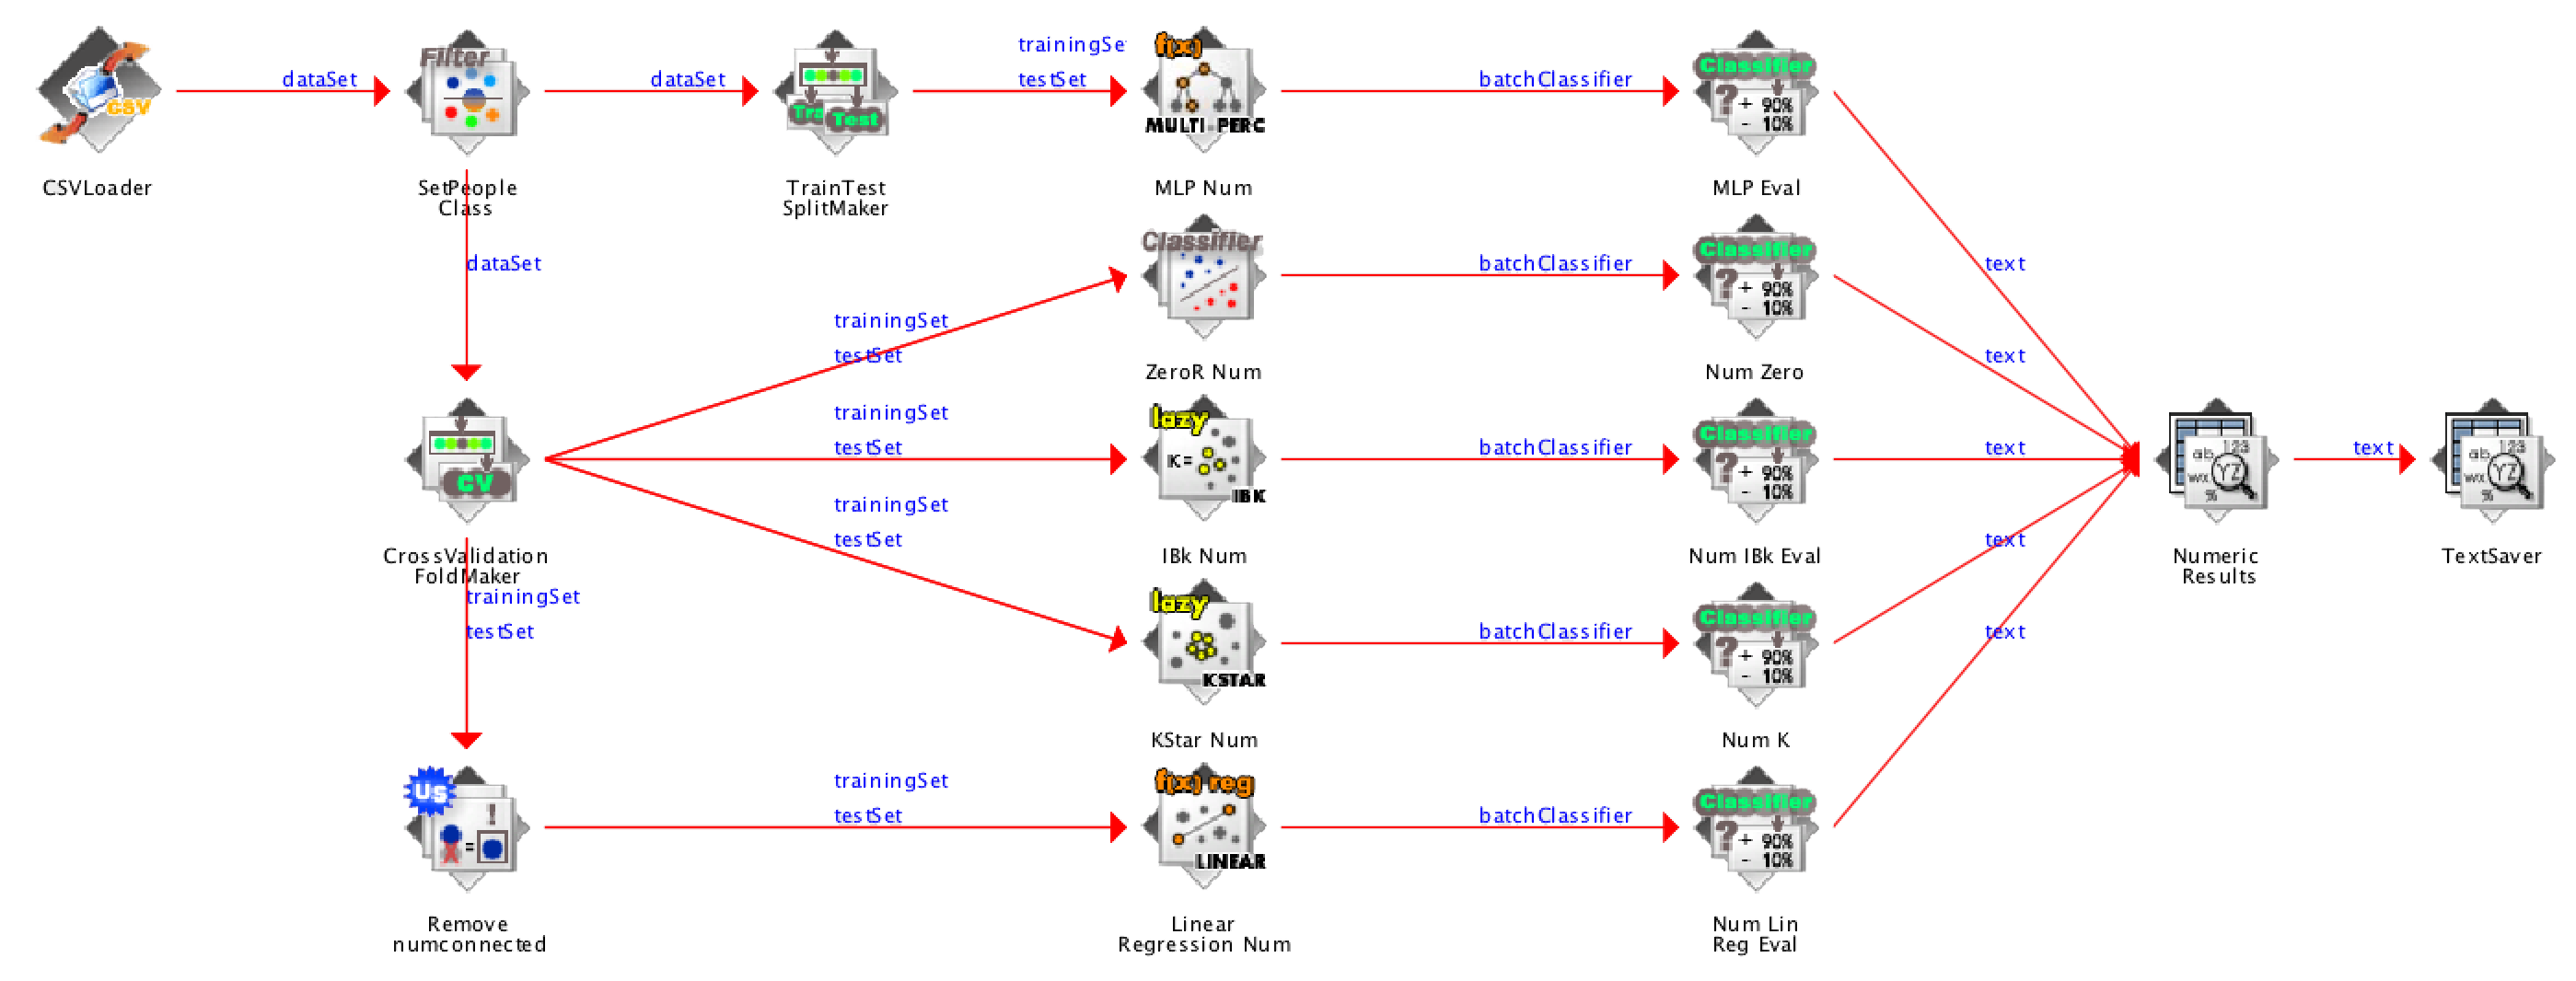
\includegraphics[width=\linewidth]{../diagrams/knowledgeflow-numeric.png}
\caption{Weka Knowledge flow for numeric classification techniques}
\end{figure}
\end{landscape}

\begin{landscape}
\begin{figure}[H]
\centering
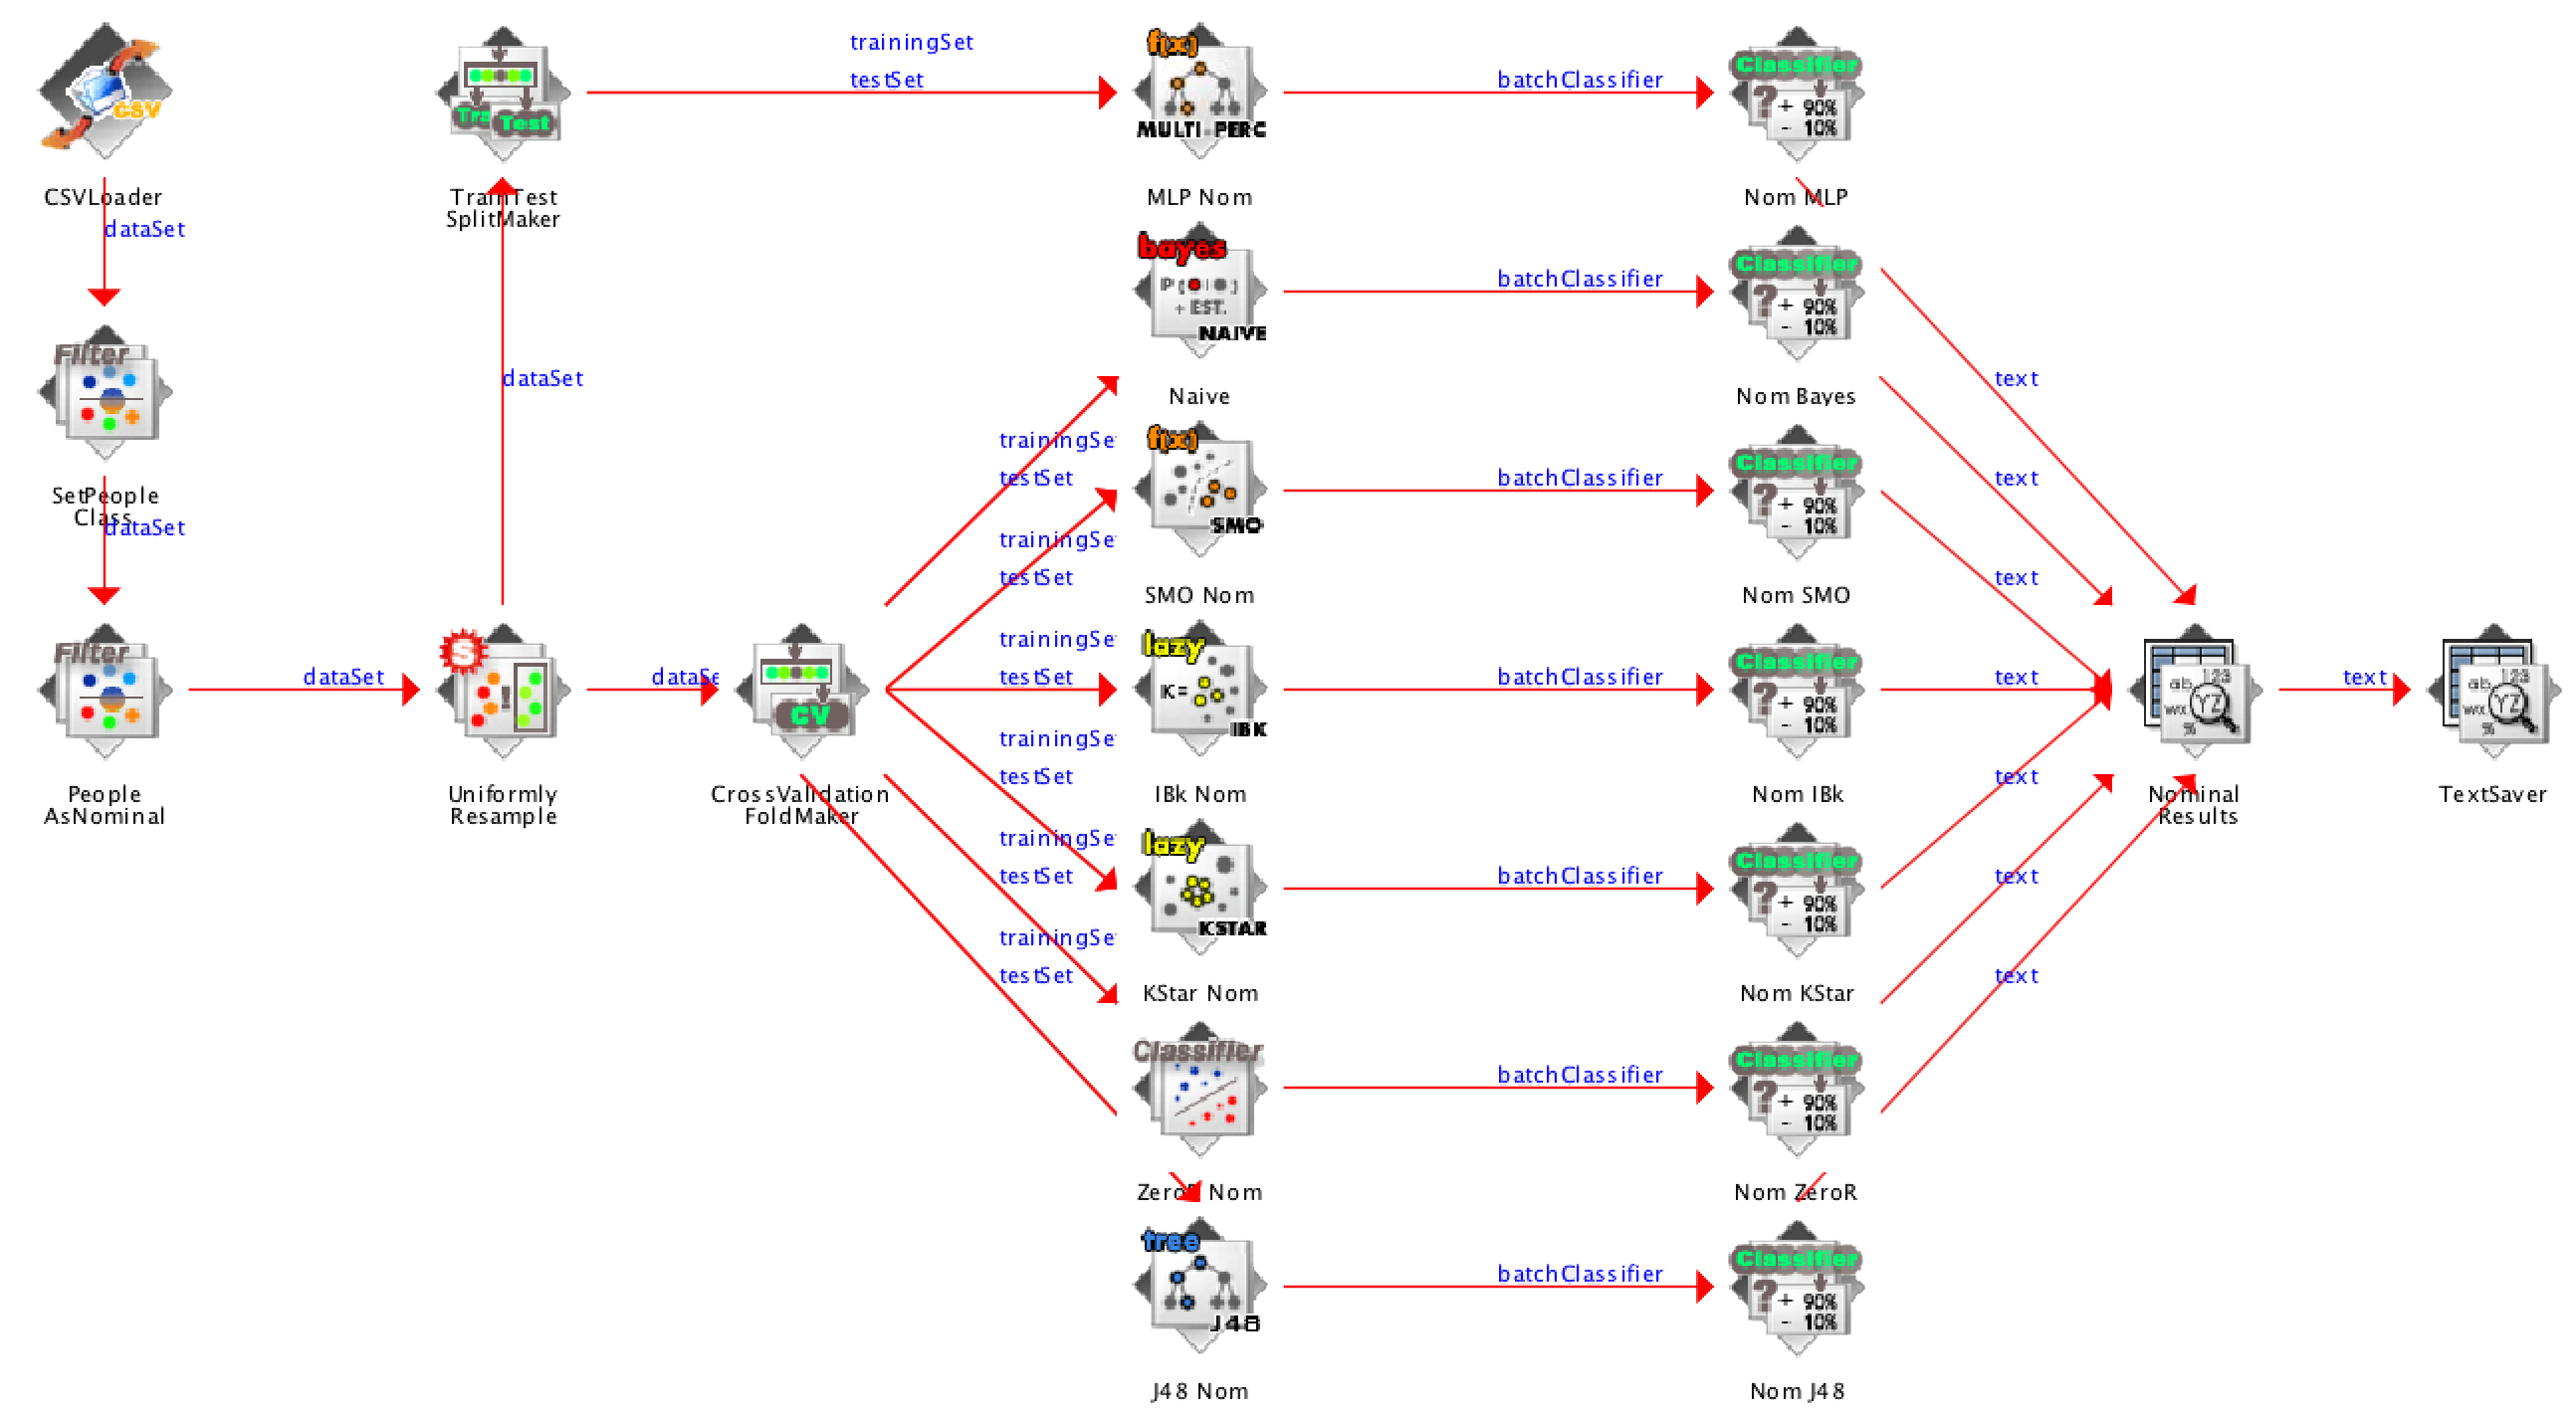
\includegraphics[width=\linewidth]{../diagrams/knowledgeflow-nominal.png}
\caption{Weka Knowledge flow for nominal classification techniques}
\end{figure}

In Weka, Knowledge Flows can be defined, which provide an easy way to replicate a series of Weka functions. We provide a unified knowledge flow in the \texttt{run\_flow.py} script to execute it on a given data set. We replicate the numeric and nominal flows separately here.
\end{landscape}

\chapter{Original Honours Proposal}
\subfile{../proposal/proposal}

%\clearpage



\end{document}


